% \section{Background}
% \subsection{Groups}
% A group \( (G, \circ) \) consists of a non-empty set \( G \) and a binary operation \(\circ: G \times G \to G\) satisfying the following axioms:
% \begin{enumerate}
%     \item \textbf{Closure:} For all \( a, b \in G \), the result of the operation \( a \circ b \) is also in \( G \): \( a \circ b \in G \).
%     \item \textbf{Identity Element:} There exists an element \( e \in G \) such that, for all \( a \in G \), \( a \circ e = e \circ a = a \).
%     \item \textbf{Associativity:} For all \( a, b, c \in G \), \( (a \circ b) \circ c = a \circ (b \circ c) \).
%     \item \textbf{Inverses:} For each \( a \in G \), there exists an element \( a^{-1} \in G \) such that \( a \circ a^{-1} = a^{-1} \circ a = e \).
% \end{enumerate}

% In general, not all groups are abelian. That is, the binary operation \(\circ\) does not necessarily commute:  
% \[
% g \circ h = h \circ g, \quad \forall g,h \in G.
% \]

% \subsection{Group Representations}
% A group representation is a homomorphism  \(\rho: G \to GL(V)\) that assigns an \(n \times n\) matrix to each group element \(g \in G\), realizing it as a linear transformation. Representations must preserve the binary operation for all members of the group \(G\) such that:
% \[
% \rho(g \circ h) = \rho(g) \rho (h), \quad \forall g,h \in G.
% \]

% A representation is reducible if it can be represented as the direct sum of other representations:
% \[
% \rho(g) = \rho_1(g) \oplus \rho_2(g), \quad \forall g \in G.
% \]

% For example, a reducible \(4 \times 4\) representation of \(SU(2)\) can be decomposed into two \(2 \times 2\) subrepresentations:

% \[
% \rho(g) =
% \begin{bmatrix}
% \rho_1(g) & 0 \\
% 0 & \rho_2(g)
% \end{bmatrix}, \quad \forall g \in SU(2),
% \]

% where \(\rho_1(g)\) and \(\rho_2(g)\) are the following irreducible representations of \(SU(2)\):

% \[
% \rho_1(g) =
% \begin{bmatrix}
% e^{i\theta} & 0 \\
% 0 & e^{-i\theta}
% \end{bmatrix}, \quad
% \rho_2(g) =
% \begin{bmatrix}
% e^{i\phi} & 0 \\
% 0 & e^{-i\phi}
% \end{bmatrix}.
% \]
% By contrast, irreducible representations or \textit{irreps} cannot be represented as a direct sum. Formally, they have no non-trivial invariant subspaces \(W \subset V\) such that:
% \[
% \rho(g)W \subset W, \quad \forall g \in G.
% \]
% Representing inputs as irreps ensures equivariance by constraining each feature to transform predictably under group actions. Given \( V = \bigoplus_{i} V_i \) with irreps \( V_i \), the transformation of an input \( x \in V \) under \( g \in G \) is:  
% \[
% \rho(g)x = \bigoplus_{i} \rho_i(g)x_i.
% \]  
% Each component \( x_i \) transforms independently according to \(\rho_i\), preserving symmetry. Scalars remain invariant, while vectors rotate according to standard representations. This decomposition prevents the mixing of differently transforming features, ensuring that all subsequent operations, linear or non-linear, respect the group’s symmetry, thereby maintaining equivariance throughout the network.

% \subsection{Tensor Products}
% \label{sec:tensor_products}
% Schur's lemma implies that there are no non-trivial linear equivariant maps that mix features decomposed into irreps. Specifically, for irreps \(\rho_i\) and \(\rho_j\), any linear map \(T: V_i \to V_j\) satisfying  
% \[
% T \rho_i(g) = \rho_j(g) T, \quad \forall g \in G,
% \]
% is either the zero map or an isomorphism if \(\rho_i \not\cong \rho_j\). Consequently, direct linear mixing between features transforming under distinct irreps is prohibited.

% Tensor products are employed to enable equivariant mixing. Given features \(x_i \in V_i\) and \(x_j \in V_j\), their tensor product \(x_i \otimes x_j\) transforms as 
% \[
% x_i \otimes x_j \mapsto (\rho_i \otimes \rho_j)(g)(x_i \otimes x_j) = \rho_i(g) x_i \otimes \rho_j(g) x_j,
% \]
% where \((\rho_i \otimes \rho_j)(g) = \rho_i(g) \otimes \rho_j(g)\). The resulting reducible representation decomposes into a direct sum of irreps:
% \[
% V_i \otimes V_j \cong \bigoplus_{k} V_k.
% \]
% This decomposition introduces new irreps \(V_k\) that permit non-trivial equivariant interactions. By projecting onto these irreps, networks can achieve feature mixing while preserving symmetry constraints.

% \subsection{Spherical Harmonics}
% Analogous to the Fourier series on the unit sphere, spherical harmonics \(Y_j\) form an orthonormal basis for the Hilbert space of square-integrable functions defined on the sphere \(L^2(S^2)\). Any function \(f(x) \in L^2(S^2)\) can be expressed in terms as:
% \begin{equation}
%     f(x) = \sum_{J \geq 0} \mathbf{f}_{J}^{\top}Y_{J},
% \end{equation}
% where the vector of coefficients \(f_J\) can be obtained via:
% \begin{equation}
%     \mathbf{f}_J = \int_{S^2}f(x)Y_{J}^*(x)dx.
% \end{equation}

% The spherical harmonics exhibit a predictable transformation property under rotations. For a rotation \(g \in G\), represented by the operator \(R_g\) on the sphere, they transform as:
% \begin{equation}
%     Y_J(R_g^{-1}x) = D_J^*(g) Y_J(x),
% \end{equation}
% where \(x \in S^2\). Here, \(D_J^*(g)\) is the complex conjugate of the \(J\)-th Wigner-D matrix, which acts on the \((2J+1)\)-dimensional space of harmonics of degree \(J\).

\section{Datasets}
\label{sec:dataset_construction}
\subsection{Model Inputs and the Dataloader}
We broadly follow \cite{shi_learning_2021, xu_equivariant_2024} in our dataset construction. We model hydrogen atoms implicitly and concatenate the position and velocity norms for each node \(i\) with their respective vectors. Unlike their implementations, we avoid explicit graph construction and do not include edge labels describing atomic bond types.

We reimplement the MD17 dataloader with a focus on improved throughput. Unlike previous versions~\cite{huang_equivariant_2022, xu_equivariant_2024}, which duplicate each input frame \(\mathcal{G}^{(t)} \to \{\mathcal{G}^{(t)}\}^{P}\) during every forward pass, our implementation performs this duplication and graph construction (if desired) during initialization. These modifications improve dataloader throughput by \(>5 \times\). The code is available at: \textbf{Anonymized for review}
% \url{https://github.com/luke-a-thompson/gtno_py/blob/main/src/gtno_py/dataloaders/egno_dataloder.py}

\begin{table}[ht]
    \centering
    \caption{Mean time (seconds) to produce \(10\ 000\) batches over \(100\) benchmark runs. Batch size \(= 100\), \(500\) samples, \(\Delta t = 3000\). We allow \(500\) warmup batches and report \(2\sigma\) confidence intervals.}
    \label{tab:dataloader_perf}
    \begin{tabular}{lcccc}
        \toprule
         & Aspirin & Ethanol & Naphthalene & Toluene \\
         \midrule
         \gls{egno} & \(0.060{\scriptstyle \pm0.024}\) & \(0.024{\scriptstyle \pm0.016}\) & \(0.056{\scriptstyle \pm0.024}\) & \(0.039{\scriptstyle \pm0.024}\) \\
         \gls{atoms} & \(0.005{\scriptstyle \pm0.002}\) & \(0.007{\scriptstyle \pm0.002}\) & \(0.008{\scriptstyle \pm0.004}\) & \(0.006{\scriptstyle \pm0.002}\) \\
         \bottomrule
    \end{tabular}
\end{table}

\subsection{Dataset Generation Algorithm}
We compute TG80 with the same PBE functional used for MD17 and RMD17, augmenting it with state-of-the-art \(\Delta 4\) dispersion corrections; as \Cref{fig:numerical_stability} illustrates, this contributes to superior numerical stability.

\subsection{DFT Theory}
\begin{table}[H]
    \centering
    \caption{An overview of the functions, dispersion correction techniques, and basis sets used in \gls{md} datasets featured.}
    \label{tab:dft_techniques}
    \begin{tabular}{lcccc}
        \toprule
        & \gls{dft} Functional & Dispersion Corrections & Basis set & Timestep \\
        \midrule
        MD17 \cite{chmiela_machine_2017} & PBE & TS & NAO & \(0.5\) fs \\
        RMD17 \cite{christensen_role_2020} & PBE & N/A & def2-SVP & \(0.5\) fs \\
        TG80 & PBE & \(\Delta 4\) & def2-SVP & \(1.0\) fs \\
        \bottomrule
    \end{tabular}
\end{table}

We evaluate the numerical stability of MD17, RMD17 and TG80. MD17 benzene clearly shows substantial centre of mass drift in \Cref{fig:MD17_numerical_quality}, which is also partially visible by the consistent motion trails shown in \Cref{fig:MD17_trajectories}. RMD17 shows much improved stability, with centre of mass drift not exceeding \(10^4\). TG80 shows the lowest drift of all datasets examined, and expectedly includes more molecules with high per-step drift (due to more complex sterically hindered geometries).
\subsection{Numerical stability}
\begin{figure}[H]
    \begin{subfigure}{0.48\textwidth}
        \centering
        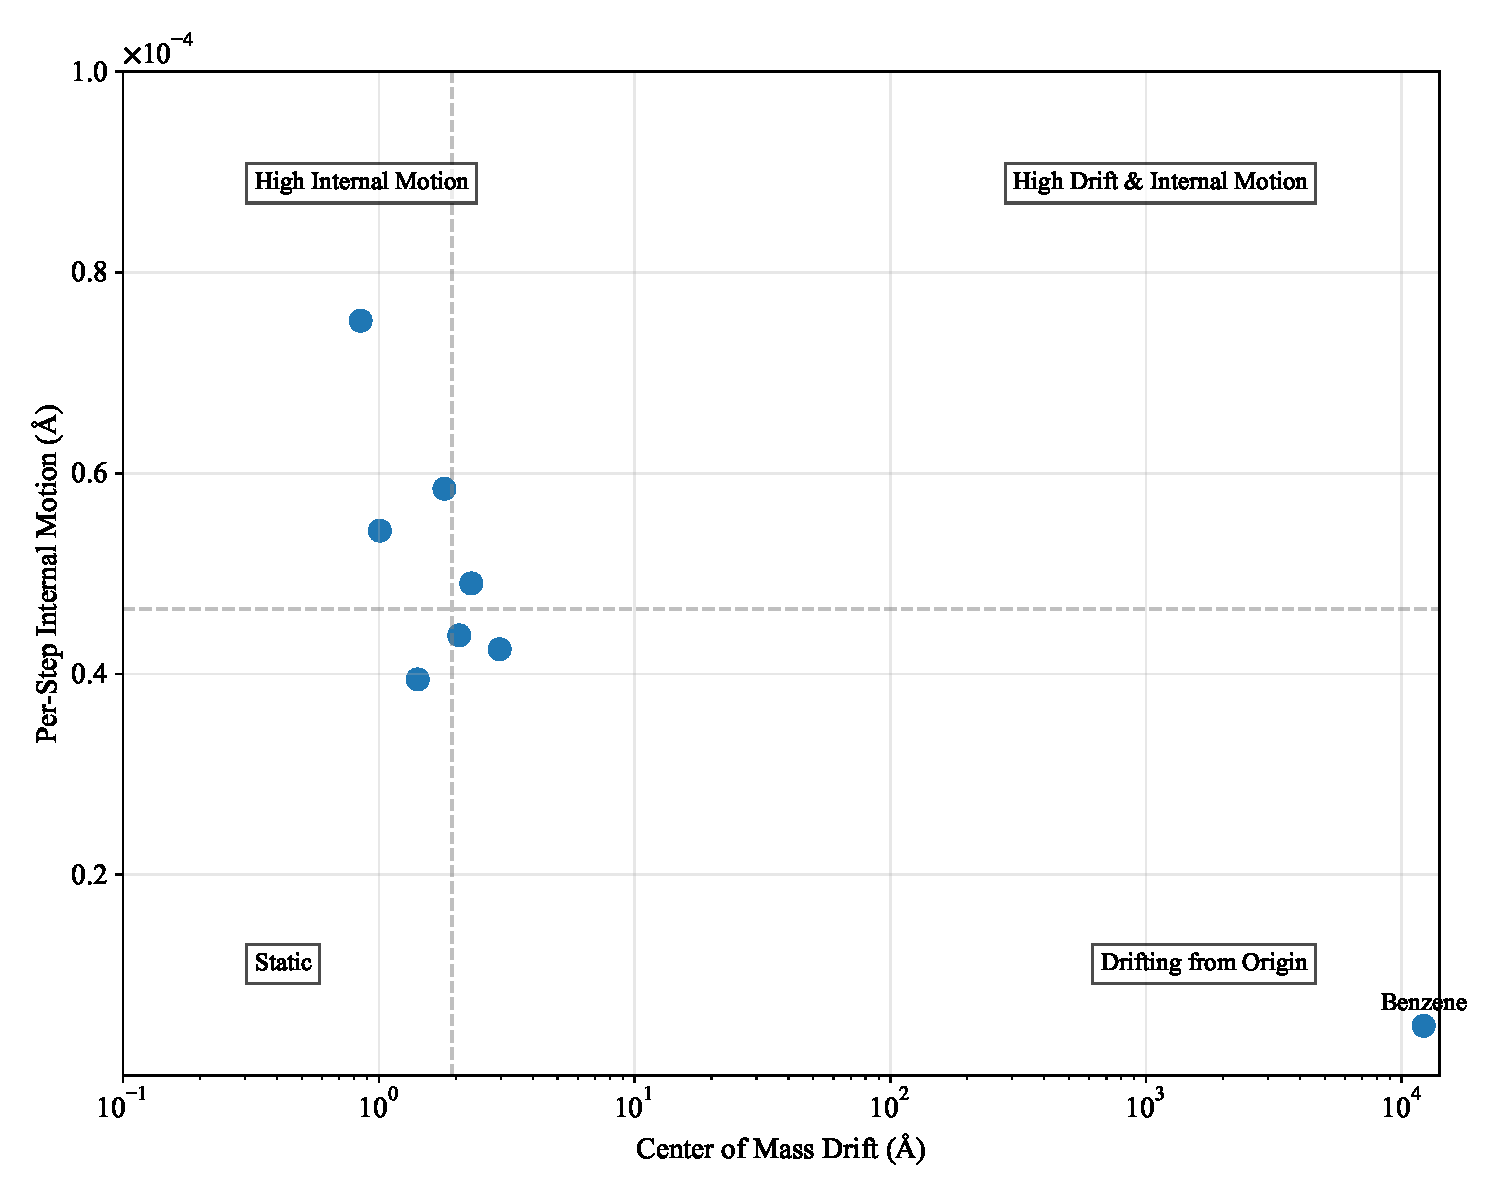
\includegraphics[width=\linewidth]{Figures/dataset/md17_molecule_behavior_comparison.pdf}
        \caption{MD17 molecules are largely consistent, save for benzene, which shows substantial drift.}
        \label{fig:MD17_numerical_quality}
    \end{subfigure}
    \hspace{0.04\textwidth}
    \begin{subfigure}{0.48\textwidth}
        \centering
        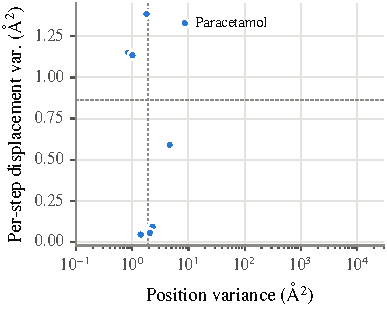
\includegraphics[width=\linewidth]{Figures/dataset/rmd17_molecule_behavior_comparison.pdf}
        \caption{RMD17 molecules exhibit improved numerical stability, supporting their use in future benchmarks.}
        \label{fig:RMD17_numerical_quality}
    \end{subfigure}
        \begin{subfigure}{0.9\textwidth}
        \centering
        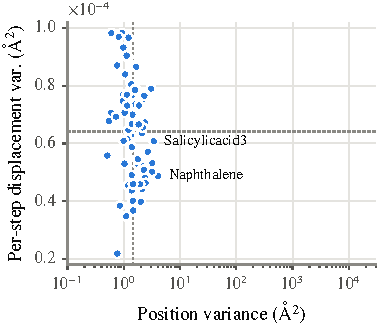
\includegraphics[width=\linewidth]{Figures/dataset/tg80_molecule_behavior_comparison.pdf}
        \caption{TG80 dataset exhibits the lowest centre-of-mass drift among the evaluated MD datasets.}
        \label{fig:TG80_numerical_quality}
    \end{subfigure}
    \caption{Comparison of numerical stability across MD17, RMD17, and TG80 datasets. Dashed lines denote the mean centre-of-mass drift and per-step motion; datapoints exceeding two standard deviations are annotated.}
    \label{fig:numerical_stability}
\end{figure}

\newpage

\subsubsection{Trajectory Samples}
\begin{figure}[H]
    \centering
    \begin{subfigure}{0.48\linewidth}
        \centering
        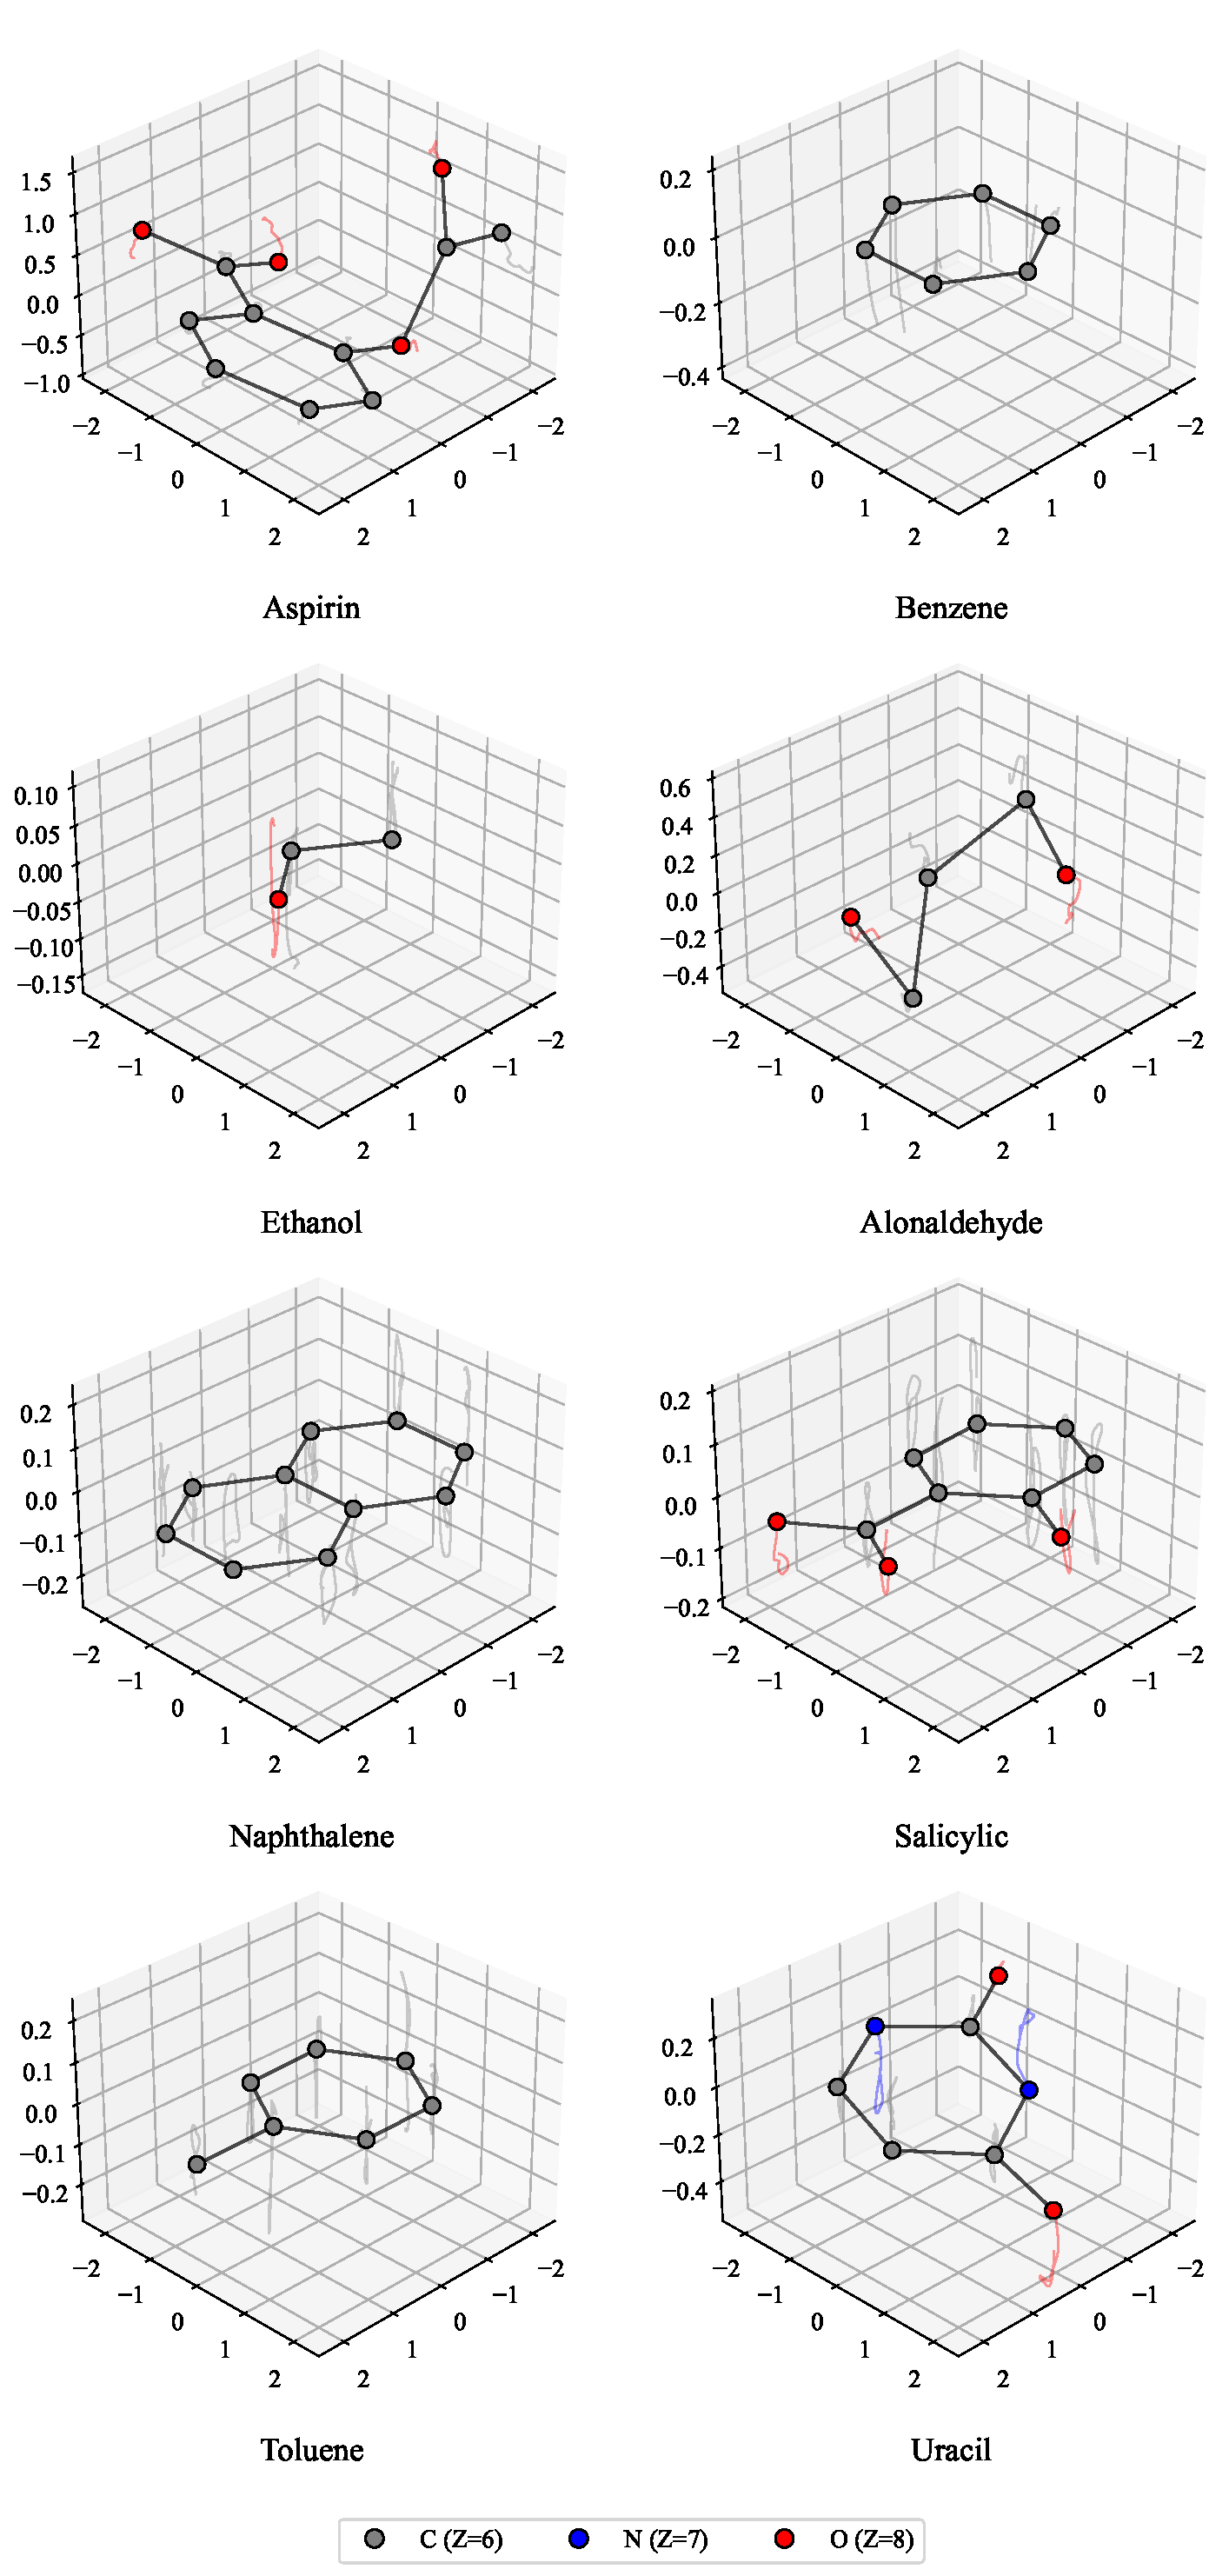
\includegraphics[width=\linewidth]{Figures/dataset/md17_combined_trajectories.pdf}
        \caption{MD17 trajectories}
        \label{fig:MD17_trajectories}
    \end{subfigure}
    \hfill
    \begin{subfigure}{0.48\linewidth}
        \centering
        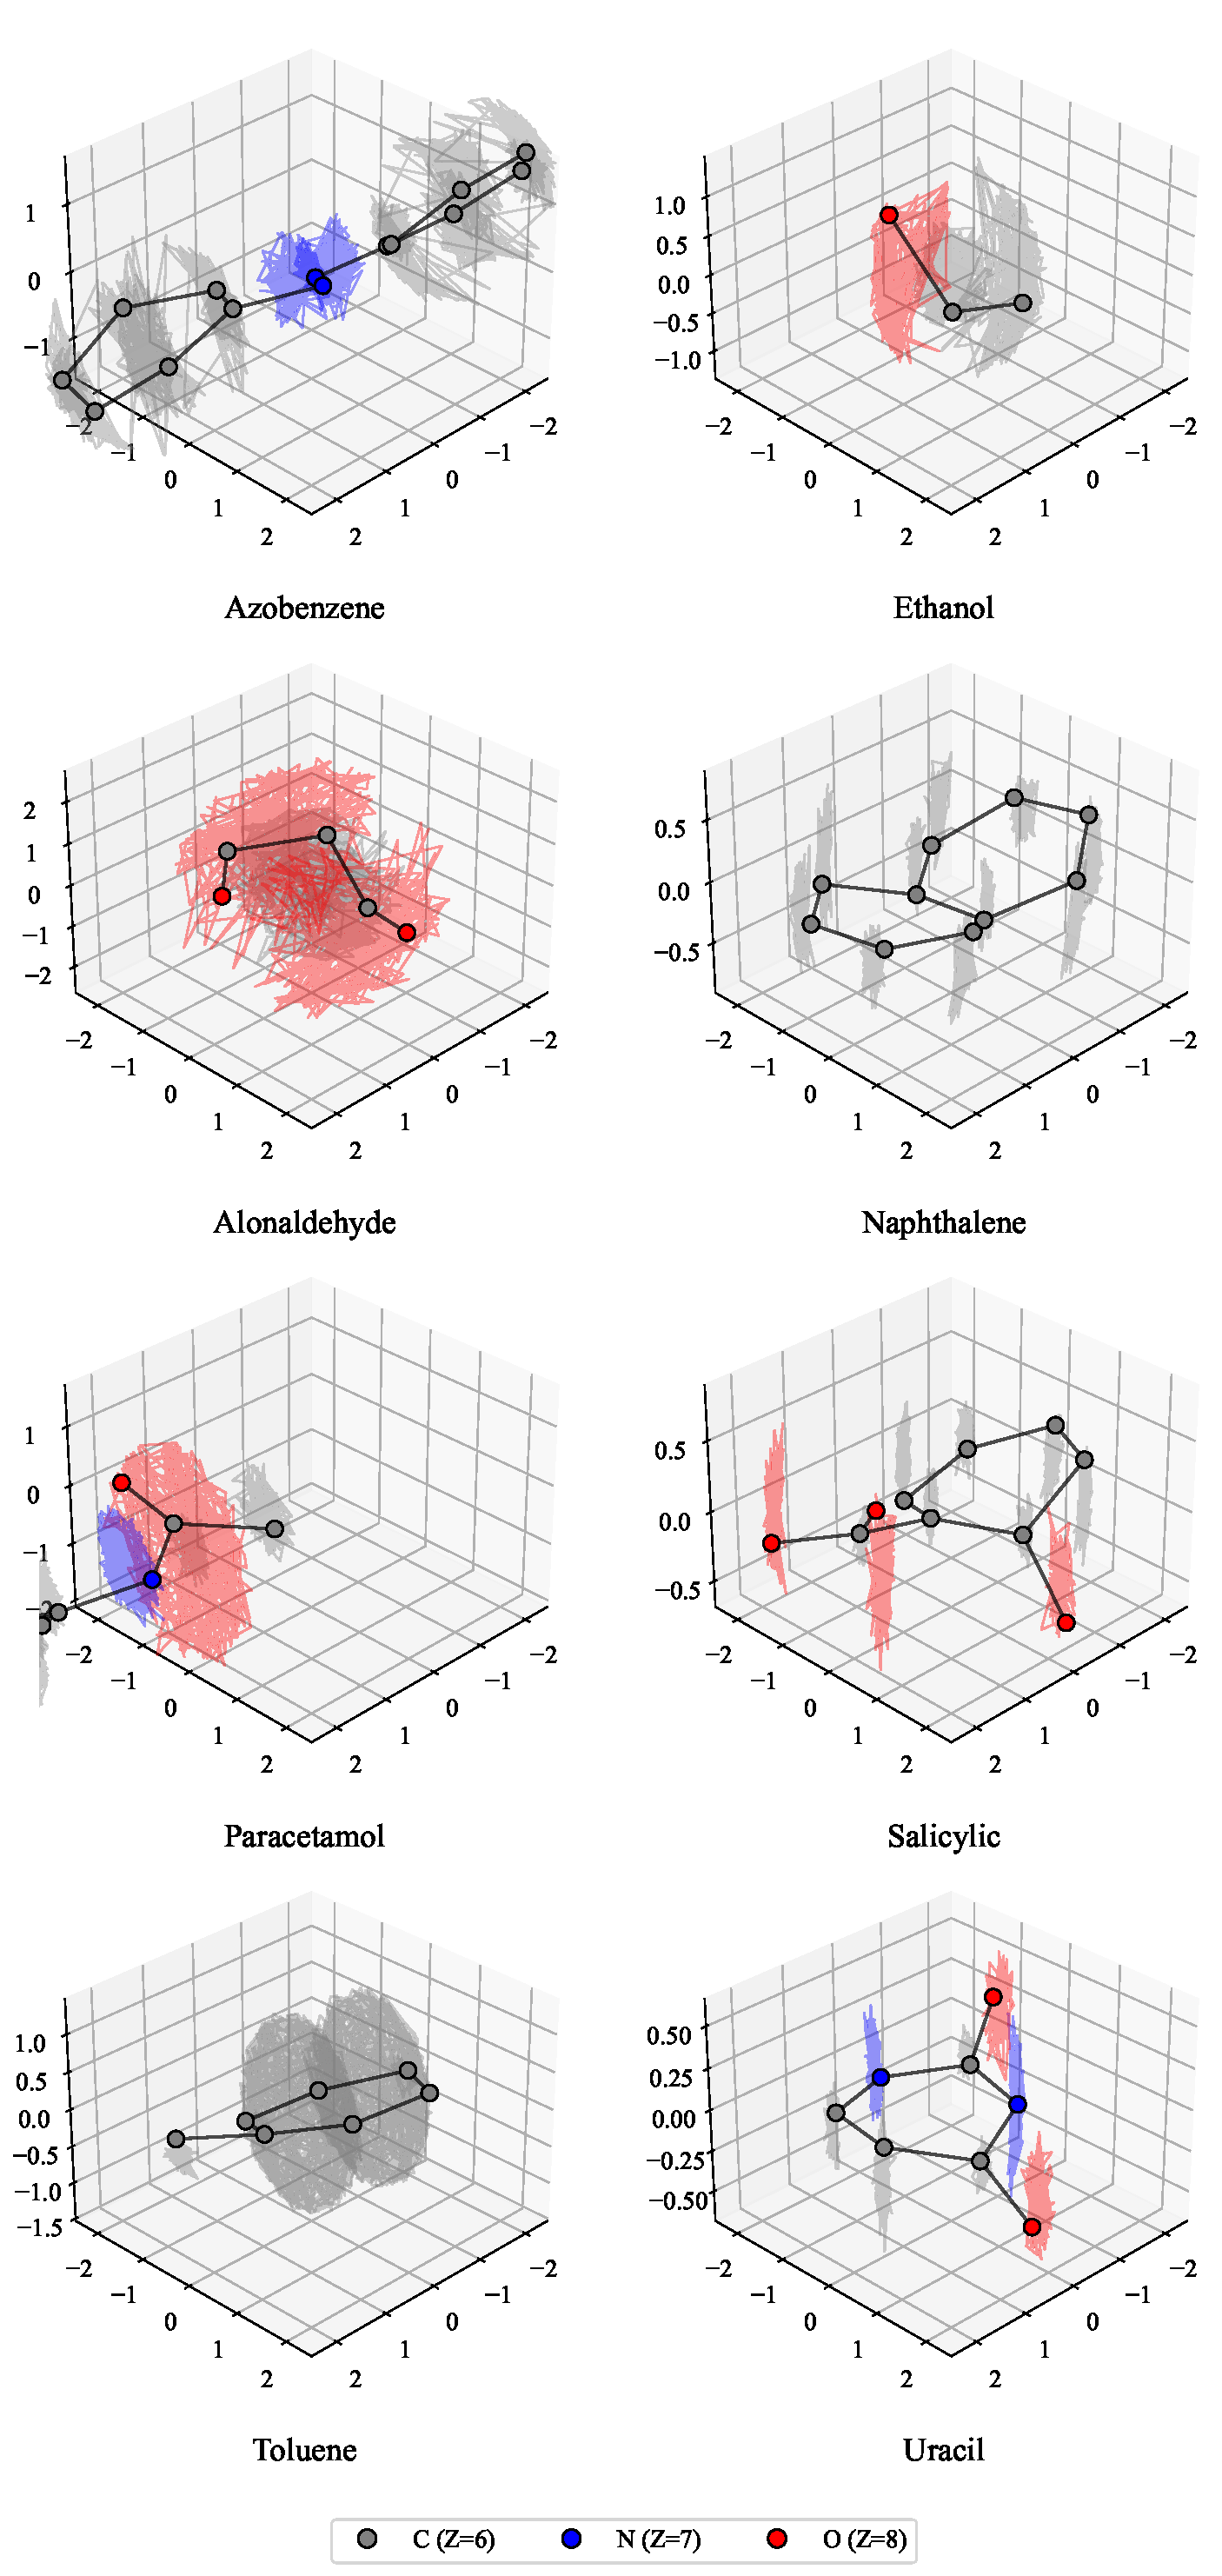
\includegraphics[width=\linewidth]{Figures/dataset/rmd17_combined_trajectories.pdf}
        \caption{RMD17 trajectories}
        \label{fig:RMD17_trajectories}
    \end{subfigure}
    \caption{3000 steps \gls{md} trajectories from the MD17 and RMD17 datasets.}
    \label{fig:trajectories}
\end{figure}

\begin{figure}[H]
    \centering
    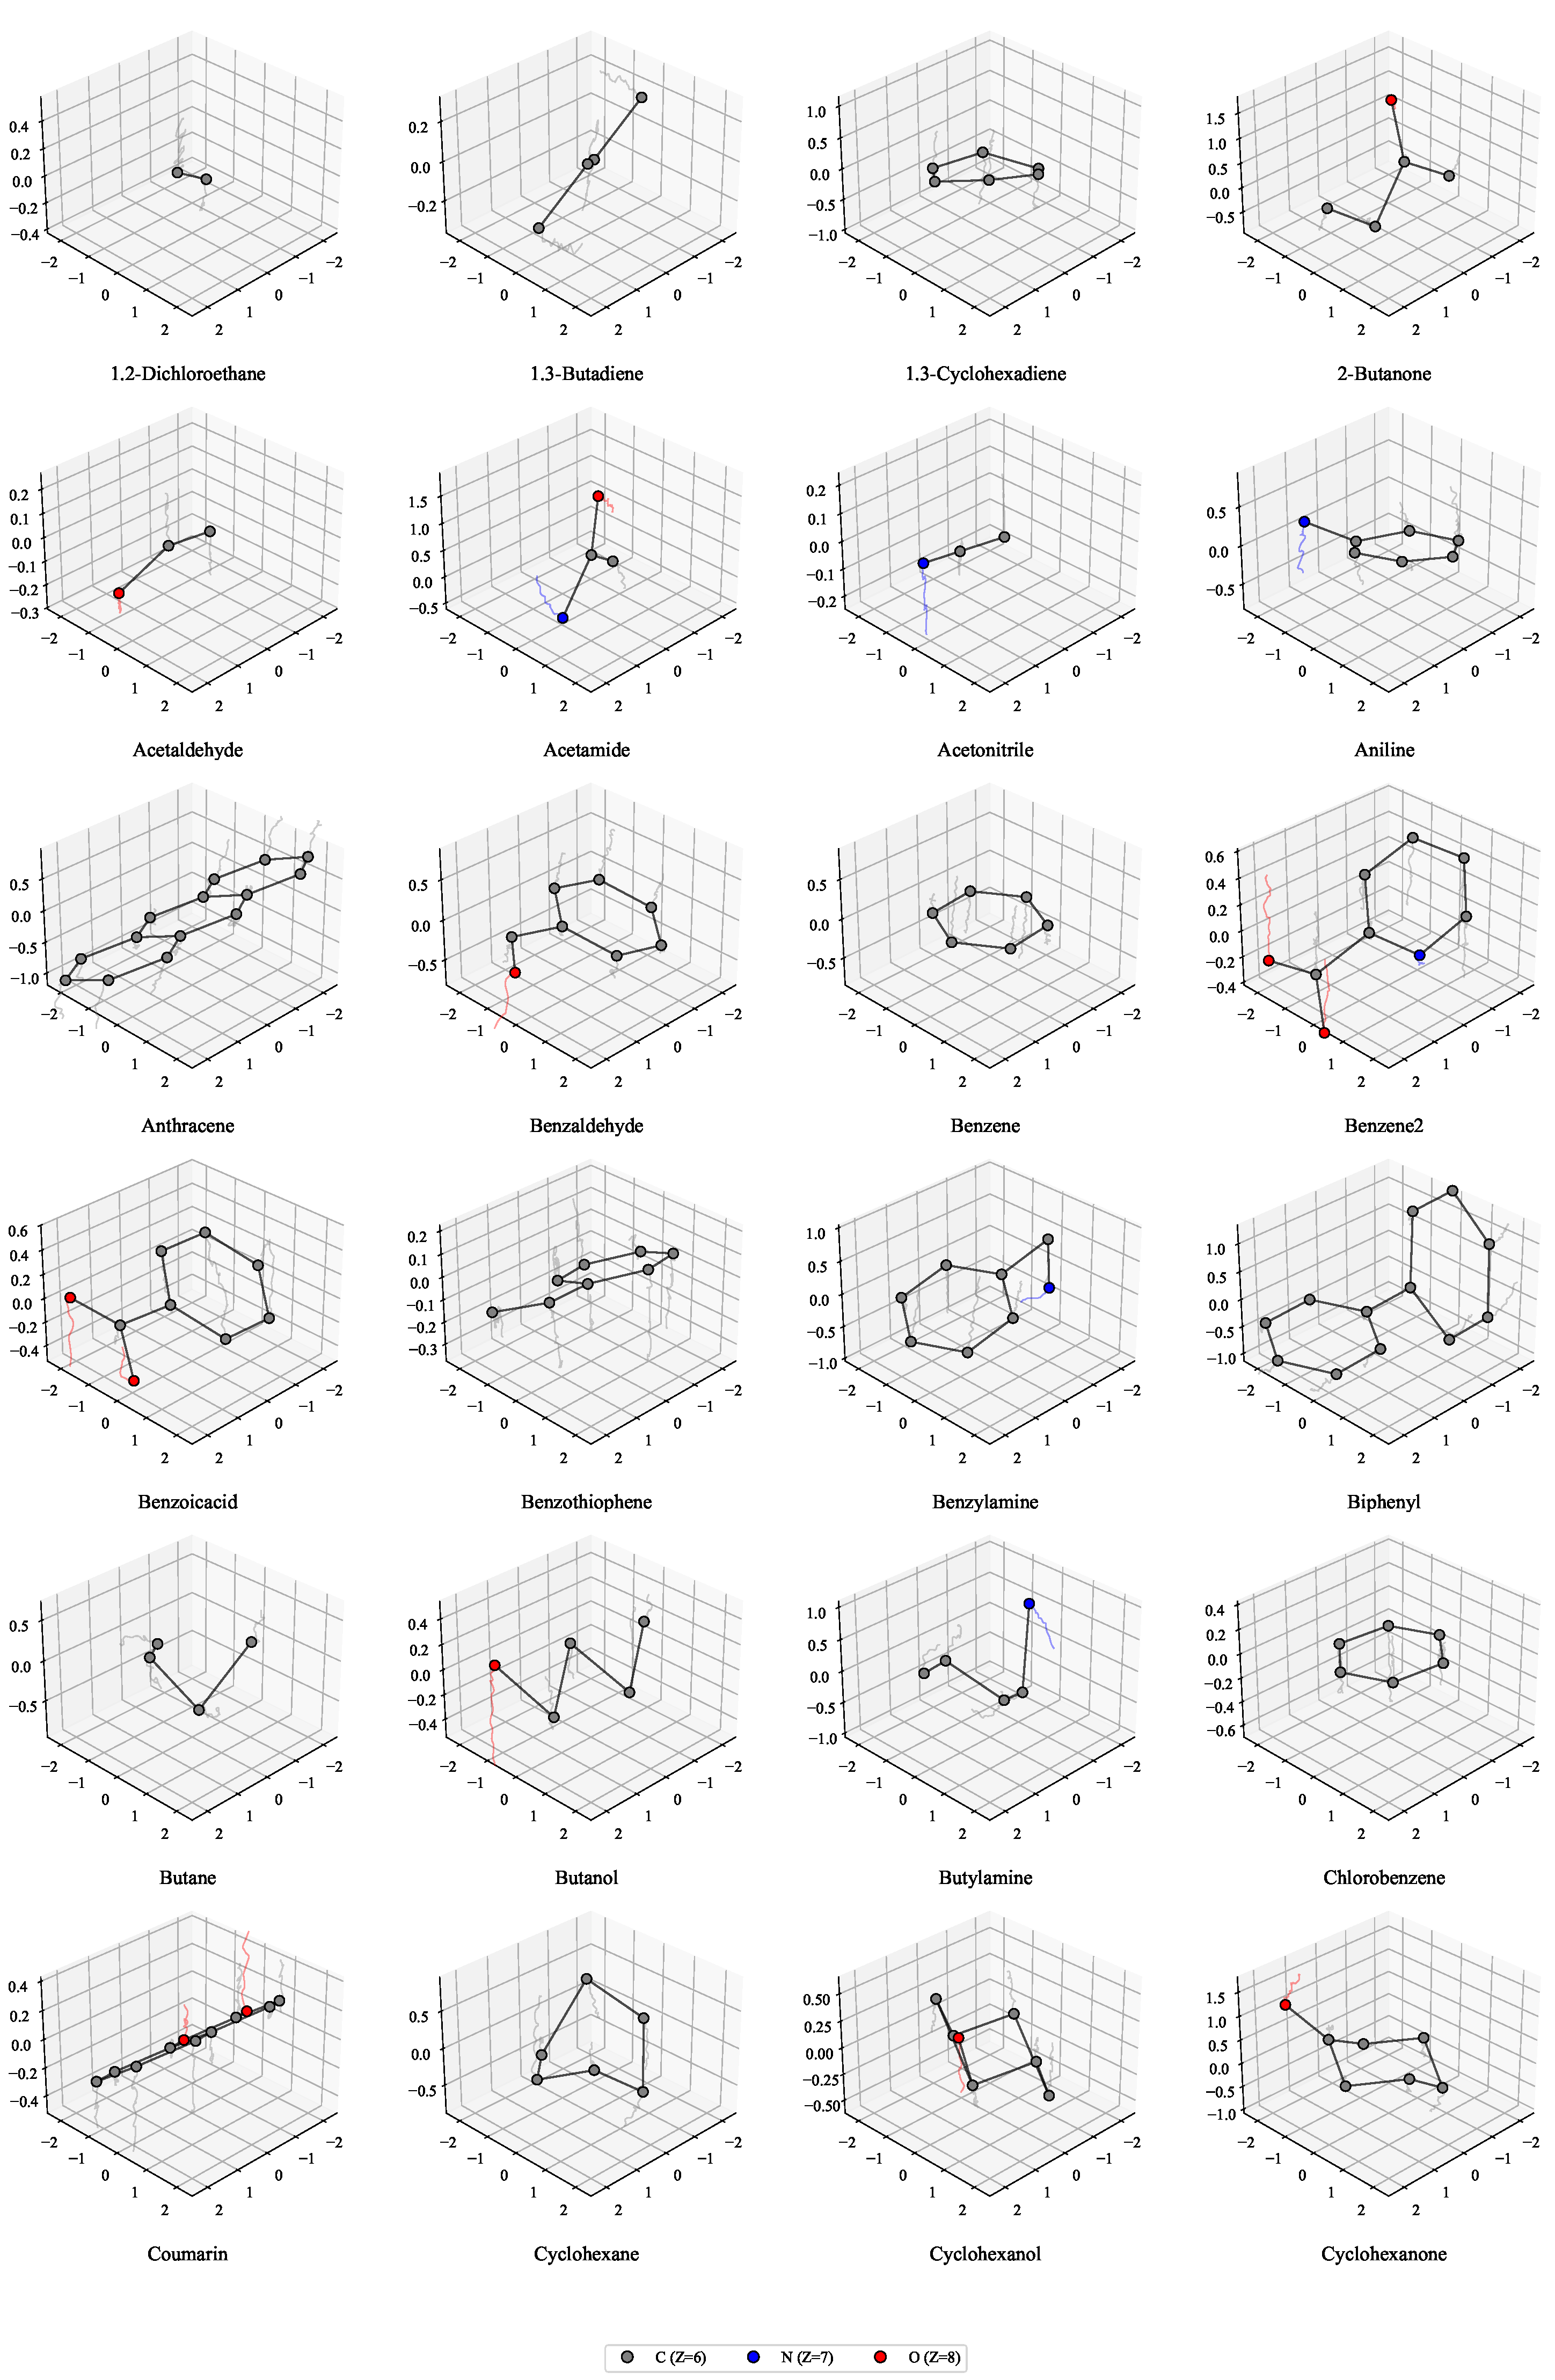
\includegraphics[width=\linewidth]{Figures/dataset/tg80_combined_trajectories_1.pdf}
    \label{fig:TG80_trajectories_1}
\end{figure}
\begin{figure}[H]
    \centering
    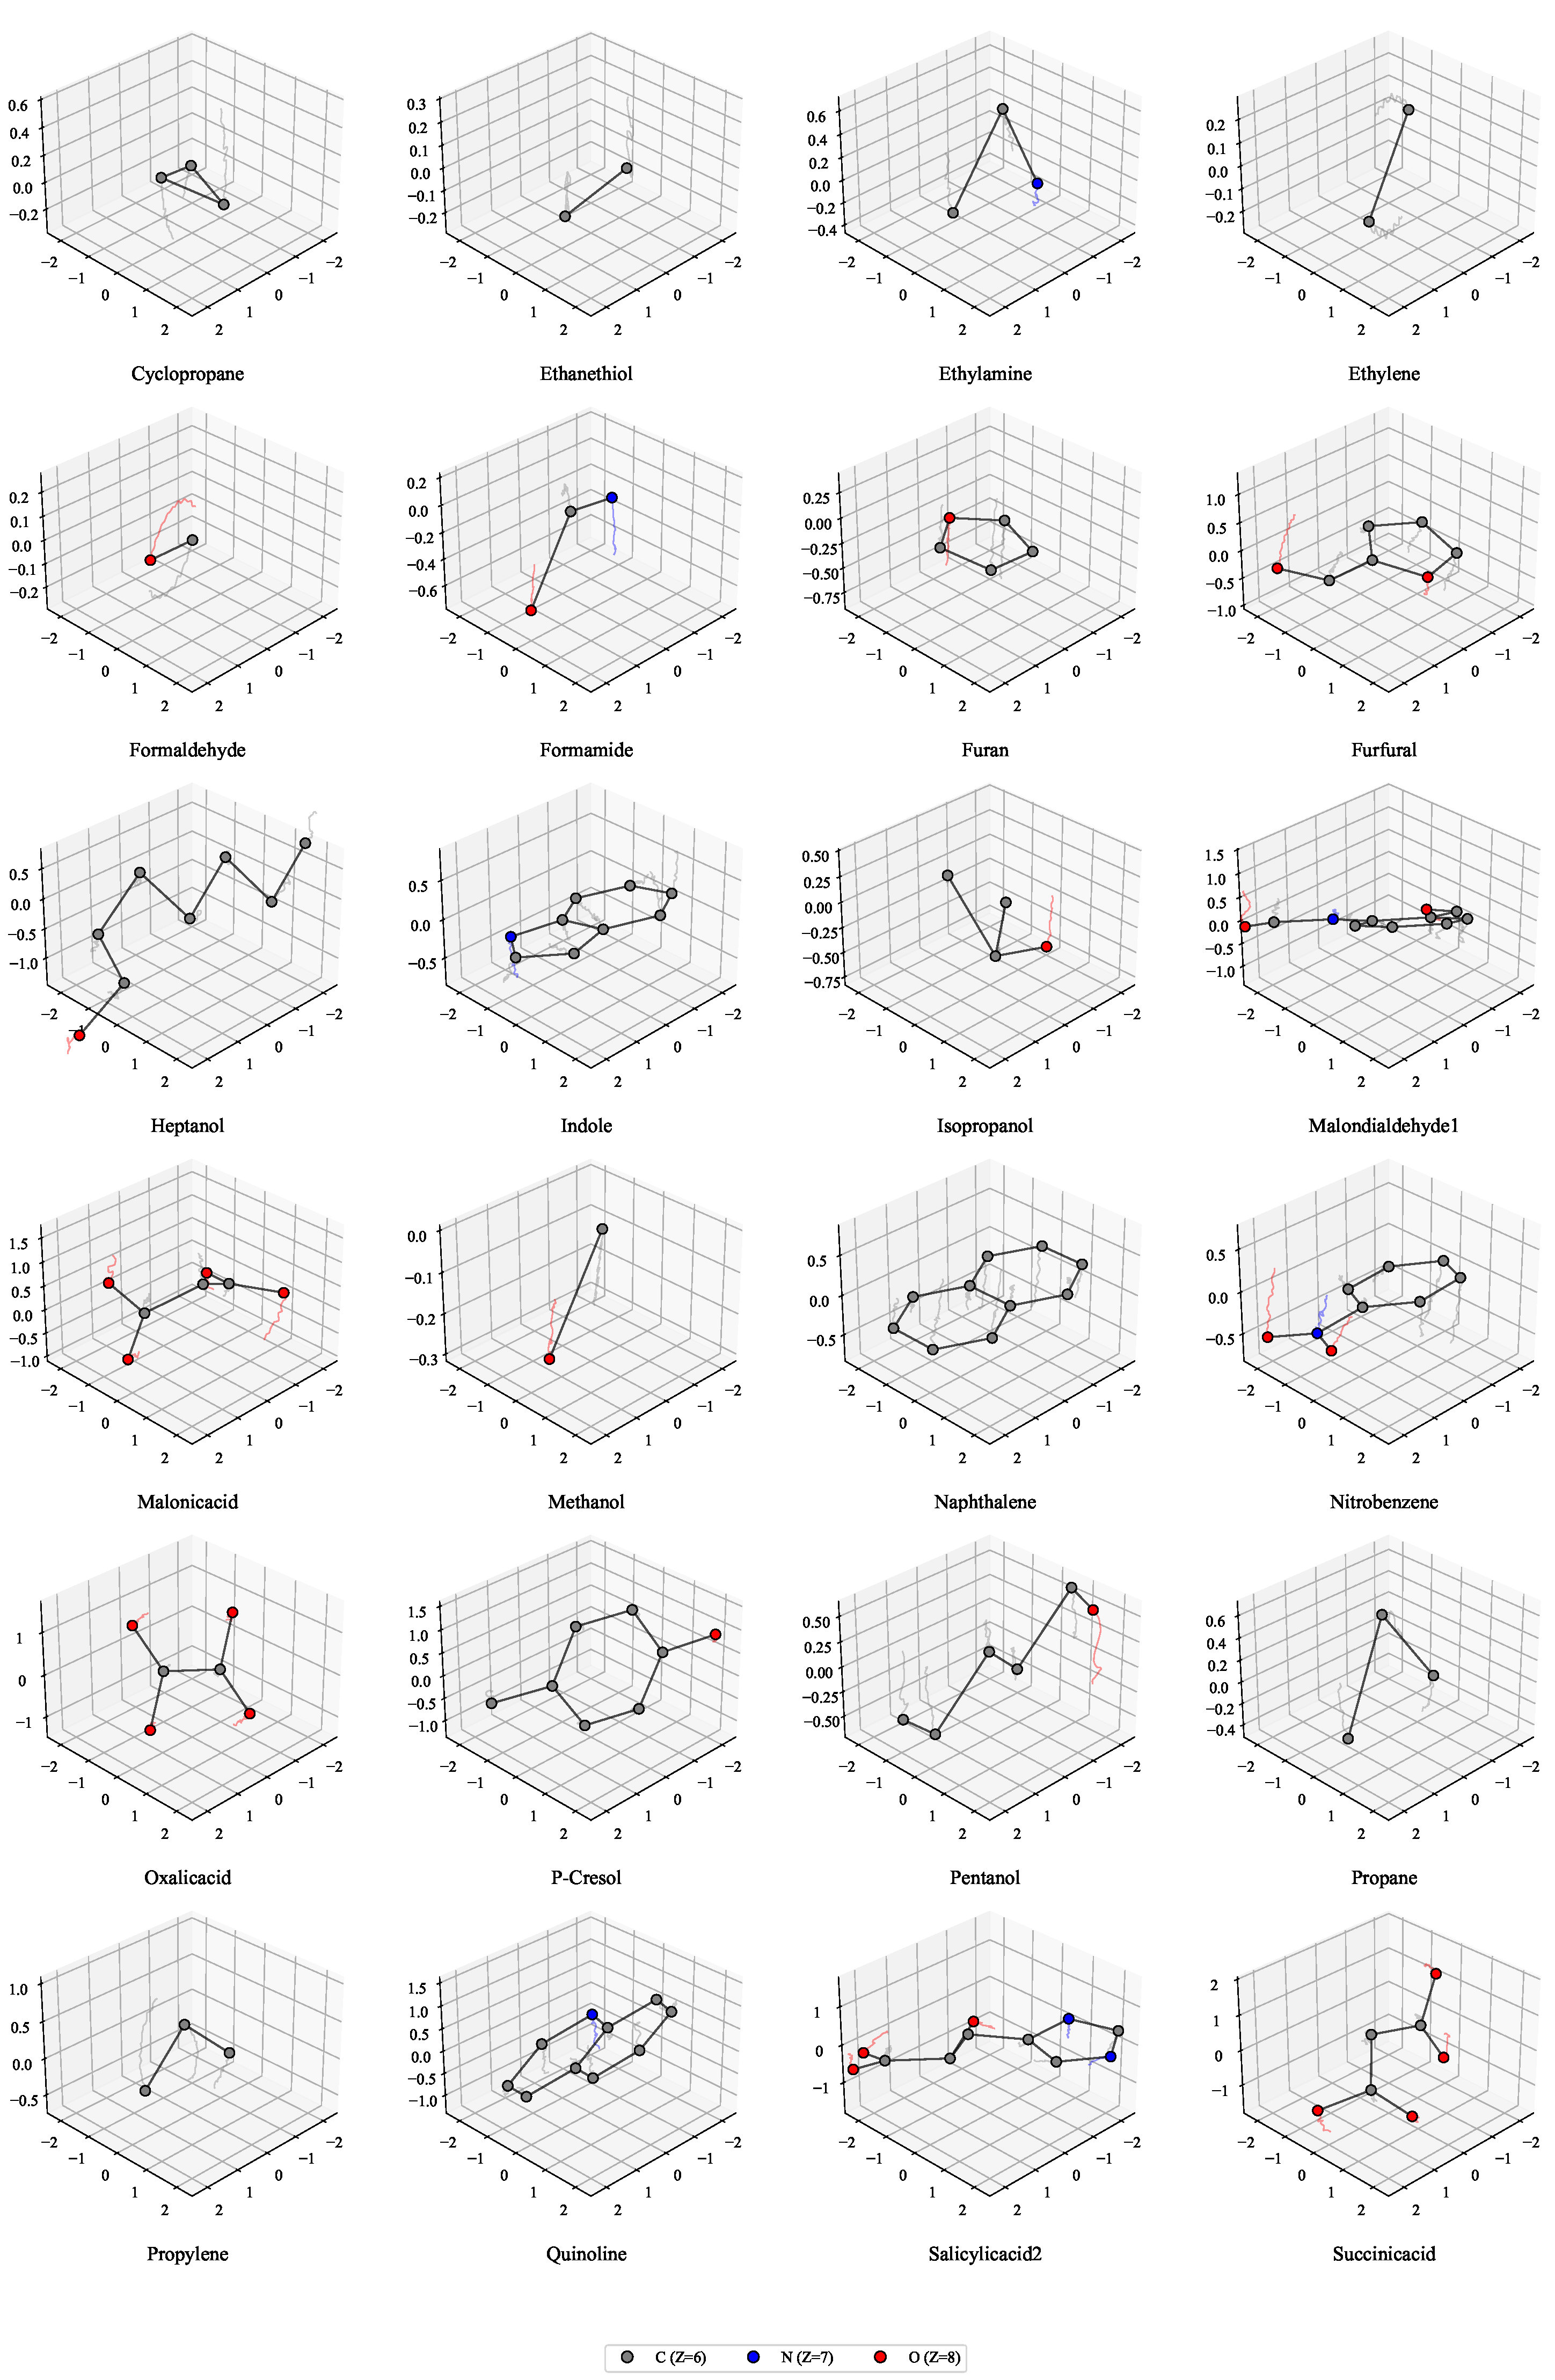
\includegraphics[width=\linewidth]{Figures/dataset/tg80_combined_trajectories_2.pdf}
    \label{fig:TG80_trajectories_2}
\end{figure}
\begin{figure}[H]
    \centering
    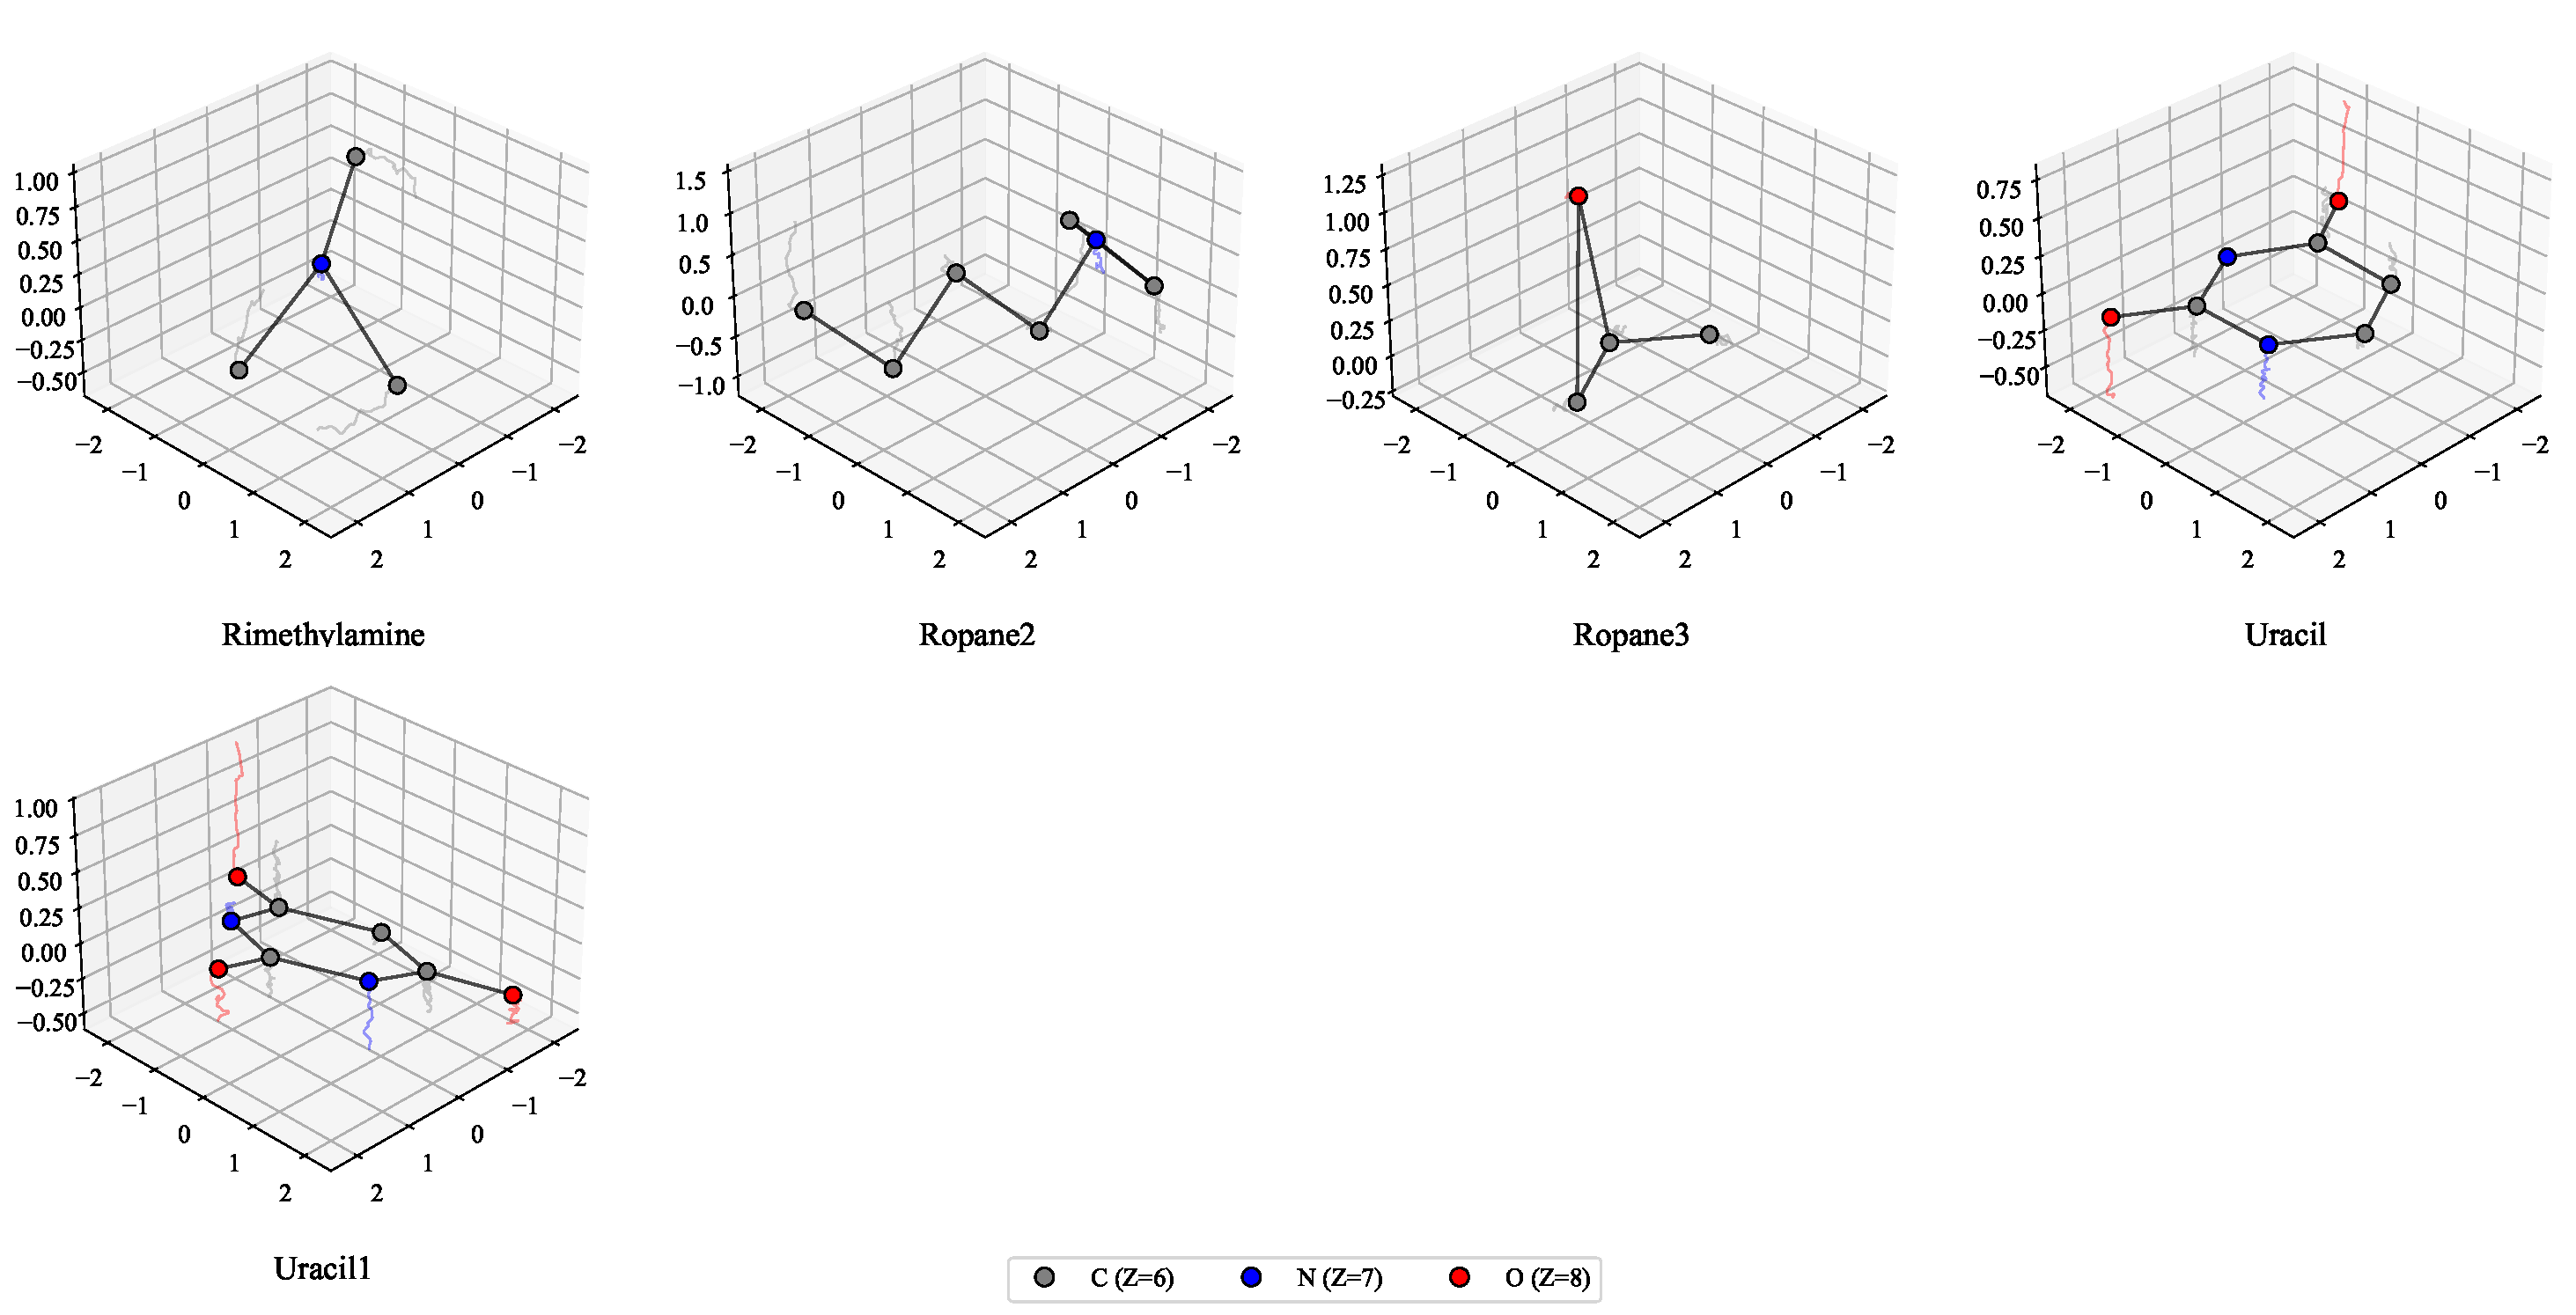
\includegraphics[width=\linewidth]{Figures/dataset/tg80_combined_trajectories_3.pdf}
    \label{fig:TG80_trajectories_3}
    \caption{3000 steps \gls{md} trajectories from the TG80 dataset. Molecules derived from our dataset expansion algorithm are named according to the seed molecule they were related to and their order of selection.}
\end{figure}

\section{Architectural Details}
\subsection{Value-residual Learning}
\label{sec:value_residuals}
We employ value-residual learning, wherein we give every transformer block access to the output of the first block via a residual connection \cite{zhou_value_2024}. This is thought to promote stable training and efficient information flow. Inspired by \cite{jordan_nanogpt_2024}, we add a learned coefficient to weight this residual. Here, \(v\) denotes the current block's value output, and \(v_1\) represents the initial block's value. A learnable parameter \(\alpha\) is passed through a sigmoid to obtain the weighting coefficient:
\begin{equation}
    \lambda = \sigma(\alpha).
\end{equation}
The combined output is then given by
\begin{equation}
    v = \lambda\,v + (1 - \lambda)\,v_1.
\end{equation}
In practice, we lock the first block's \(\lambda\) value to \(0.5\). We report the learned \(\lambda\) values in \Cref{fig:lambda_values}.

\begin{figure}[H]
    \begin{subfigure}{0.48\textwidth}
        \centering
        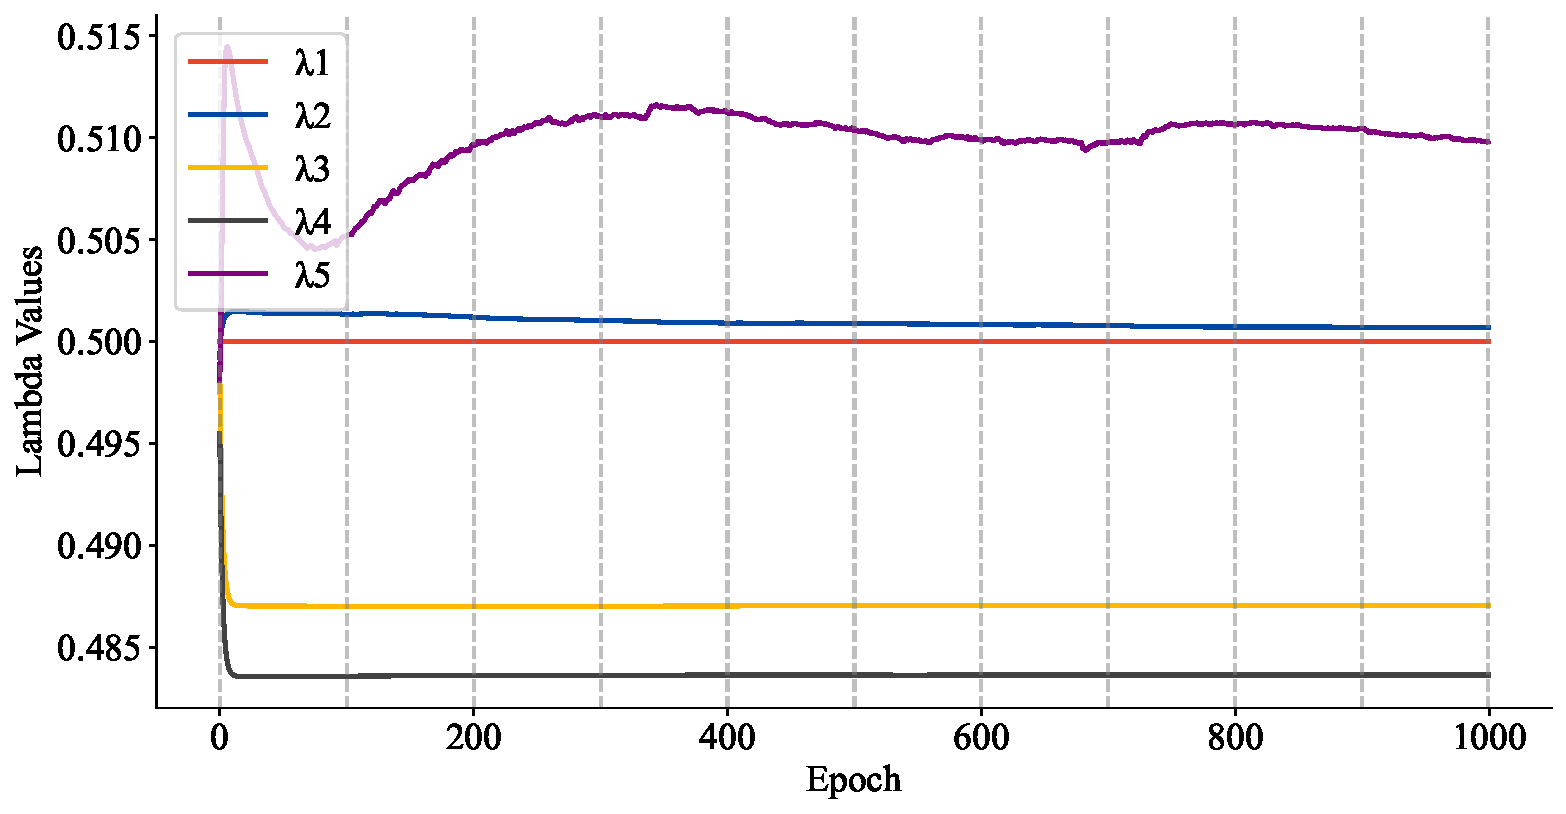
\includegraphics[width=\textwidth]{Figures/lambda_residuals/lambda_values_aspirin.pdf}
        \caption{Aspirin}
    \end{subfigure}
    \hfill
    \begin{subfigure}{0.48\textwidth}
        \centering
        \includegraphics[width=\textwidth]{Figures/lambda_residuals/lambda_values_ethanol.pdf}
        \caption{Ethanol}
    \end{subfigure}
    \begin{subfigure}{0.48\textwidth}
        \centering
        \includegraphics[width=\textwidth]{Figures/lambda_residuals/lambda_values_napthalene.pdf}
        \caption{Napthalene}
    \end{subfigure}
    \hfill
    \begin{subfigure}{0.48\textwidth}
        \centering
        \includegraphics[width=\textwidth]{Figures/lambda_residuals/lambda_values_toluene.pdf}
        \caption{Toluene}
    \end{subfigure}
    
    \caption{Learned \(\lambda\) values for each \gls{atoms} transformer block on four MD17 molecules.}
    \label{fig:lambda_values}
\end{figure}

\subsection{Delta-prediction}
\label{sec:delta_prediction}
When \(\Delta\)-prediction is enabled, as in \Cref{fig:MD17_ablation}, we incorporate the initial positions \(\mathbf{x}\) as a residual term, reformulating the model as an operator that learns a displacement field rather than predicting absolute positions. We express this as:
\begin{equation}
    \mathbf{x}^\dagger = \operatorname{Project}(\mathbf{x}_{\text{out}}) + \mathbf{x}.
\end{equation}

In practice, this strategy diminishes performance on all molecules except Benzene. We hypothesize that due to massive positional drift, the network learns to minimize its output and allow the residual to dominate.

\subsection{Multi-head Output}
\label{sec:multi_head_output}
In the multitask case, we utilize a mixture-of-experts-like system to dynamically weight the contribution of multiple output heads based on global molecular context. In this case, each head is a \(\operatorname{Project}\) \gls{mlp} identical to that described in \Cref{sec:project}.

Given a set of phase space vectors \(\{ \mathbf{z}_1, \dots, \mathbf{z}_N \} \subseteq \mathbf{Z} \), we compute the mean pool for the whole molecule:
\begin{equation}
    \bar{\mathbf{z}} = \frac{1}{N} \sum\limits_{\mathbf{z} \in \mathbf{Z}} \mathbf{z}.
\end{equation}
We pass this mean pooled representation through a gating network \(\operatorname{ProjectGate} \colon \mathbb{R}^d \to \mathbb{R}^{\text{n\_proj}}\) where \(\text{n\_proj}\) is the number of \(\operatorname{Project}\) heads. A softmax then generates the head weights:
\begin{equation}
    \mathbf{w} = \operatorname{softmax}(\operatorname{HeadGate}(\bar{\mathbf{z}})),
\end{equation}

This then weights the contribution of each \(\operatorname{Project}\) head to the final output:

\begin{align}
    \mathbf{x}_i^\dagger& = \operatorname{Project}_i(\mathbf{x}_\text{out})
    \\
    \mathbf{x}^\dagger &= \sum\limits_{i=1}^{\text{n\_proj}} w_i \cdot \mathbf{x}_i^\dagger
\end{align}

In the single-task learning case, the update remains exactly as described in \Cref{sec:project}.

\section{Further Experiments}
\paragraph{Revised MD17 Dataset}
Using the same dataset parameters as for MD17, we find the performance of \gls{atoms} remains excellent on the denoised revised MD17 (RMD17) dataset, with the most substantial improvement seen on naphtalene \cite{christensen_revised_2020}. Performance is generally more consistent, with fewer major regressions vs \gls{egno}.

\begin{table}[H]
    \centering
    \caption{MSE (\(\times 10^{-2}\)) on RMD17. Upper part: S2S \gls{mse}. Lower part: S2T \gls{mse}}
    \label{tab:rmd17_results}
    \resizebox{\linewidth}{!}{
    \begin{tabular}{lccccccccc}
        \toprule
        & Azobenzene & Ethanol & Malonaldehyde & Naphthalene & Paracetamol & Salicylic & Toluene & Uracil & Mean \% \\
        \midrule
        EGNO & \(10.82{\scriptstyle \pm0.05}\) & \(28.27{\scriptstyle \pm0.16}\) & \(49.25{\scriptstyle \pm0.10}\) & \(1.85{\scriptstyle \pm0.01}\) & \(28.90{\scriptstyle \pm0.20}\) & \(1.26{\scriptstyle \pm0.01}\) & \(28.44{\scriptstyle \pm0.18}\) & \(0.98{\scriptstyle \pm0.01}\) \\
        \gls{atoms} & \(\mathbf{8.36}{\scriptstyle \pm0.01}\) & \(\mathbf{23.81}{\scriptstyle \pm1.29}\) & \(\mathbf{39.87}{\scriptstyle \pm0.53}\) & \(\mathbf{1.42}{\scriptstyle \pm0.01}\) & \(\mathbf{28.74}{\scriptstyle \pm0.33}\) & \(\mathbf{1.09}{\scriptstyle \pm0.01}\) & \(28.48{\scriptstyle \pm0.02}\) & \(\mathbf{0.89}{\scriptstyle \pm0.01}\) \\
        \midrule
        \rowcolor{gray!20} Improvement (\%) & \(22.74\%\) & \(15.78\%\) & \(19.05\%\) & \(23.24\%\) & \(0.55\%\) & \(13.49\%\) & \(-0.14\%\) & \(9.18\%\) & \(\mathbf{12.99\%}\) \\
        
        \midrule
        EGNO & \(10.75{\scriptstyle \pm0.05}\) & \(28.19{\scriptstyle \pm0.16}\) & \(48.78{\scriptstyle \pm0.10}\) & \(1.80{\scriptstyle \pm0.01}\) & \(\mathbf{28.29}{\scriptstyle \pm0.20}\) & \(1.25{\scriptstyle \pm0.01}\) & \(28.37{\scriptstyle \pm0.18}\) & \(0.98{\scriptstyle \pm0.01}\) \\
        \gls{atoms} & \(\mathbf{8.61}{\scriptstyle \pm0.01}\) & \(\mathbf{23.48}{\scriptstyle \pm 
        0.14}\) & \(\mathbf{40.36}{\scriptstyle \pm0.33}\) & \(\mathbf{1.41}{\scriptstyle \pm0.01}\) & \(28.79{\scriptstyle \pm0.33}\) & \(\mathbf{1.08}{\scriptstyle \pm0.01}\) & \(28.45{\scriptstyle \pm0.071}\) & \(\mathbf{0.89}{\scriptstyle \pm0.01}\) \\
        \midrule
        \rowcolor{gray!20} Improvement (\%) & \(19.91\%\) & \(16.71\%\) & \(17.26\%\) & \(21.67\%\) & \(-1.77\%\) & \(13.60\%\) & \(-0.28\%\) & \(9.18\%\) & \(\mathbf{12.04\%}\) \\
        \bottomrule
    \end{tabular}
    }
\end{table}

\subsection{Explicit hydrogen representation}
We hypothesized that our model's underperformance relative to \gls{egno} on malonaldehyde was due to the omission of explicit hydrogens, limiting its ability to capture electron delocalization effects involving hydroxyl hydrogens. We tested two explicit hydrogen methods: 
\begin{enumerate}
    \item Including all hydrogens with gradients computed for all atoms during training
    \item Including all hydrogens but computing gradients only for heavy atoms
\end{enumerate}

Contrary to conventional \gls{md} practice, neither method improved heavy-atom test loss.

\begin{table}[H]
    \centering
    \caption{\gls{atoms} S2T MSE loss with implicit hydrogens and two explicit hydrogen approaches.}
    \label{tab:explicit_hydrogens}
    \begin{tabular}{lcc}
        \toprule
        & Aspirin & Malonaldehyde \\
        \midrule
        Implicit hydrogens &  \\
        Explicit hydrogens 1 & \(7.48{\scriptstyle \pm0.11}\) & \(15.15{\scriptstyle \pm0.22}\) \\
        Explicit hydrogens 2 & \(6.96{\scriptstyle \pm0.20}\) & \(13.52{\scriptstyle \pm0.10}\)\\
        \bottomrule
    \end{tabular}
\end{table}

\subsection{Learnable attention denominator}
Following \textcite{jordan_nanogpt_2025} and correspondence with the authors, we experimented with a learnable per-head attention scale and initialized it to the standard \(d_k\). Specific ablation studies on aspirin, ethanol, naphthalene, and toluene failed to improve \gls{mse} significantly. We also found that the change in values over the course of training was minimal, in the order of \(2\%\).

\begin{table}[H]
    \centering
    \caption{MSE (\(\times 10^{-2}\)) with and without learnable attention denominators across four MD17 compounds. Upper part: S2S. Lower part: S2T.}
    \label{tab:att_denom}
    \begin{tabular}{lcccc}
        \toprule
        & Aspirin & Ethanol & Napthalene & Toluene \\
        \midrule
         Standard & \(\mathbf{6.52}{\scriptstyle \pm0.04}\) & \(\mathbf{3.47}{\scriptstyle \pm0.05}\) & \(\mathbf{0.40}{\scriptstyle \pm0.01}\) & \(4.68{\scriptstyle \pm0.17}\) \\
         Learnable denom & \(6.89{\scriptstyle \pm0.21}\) & \(3.65{\scriptstyle \pm0.12}\) & \(0.41{\scriptstyle \pm0.00}\) & \(\mathbf{4.35}{\scriptstyle \pm0.24}\) \\
         \midrule
         Standard & \(\mathbf{5.45}{\scriptstyle \pm0.14}\) & \(\mathbf{2.69}{\scriptstyle \pm0.05}\) & \(\mathbf{0.37}{\scriptstyle \pm0.01}\) & \(2.26{\scriptstyle \pm0.07}\) \\
         Learnable denom & \(5.62{\scriptstyle \pm0.24}\) & \(2.81{\scriptstyle \pm0.09}\) & \(0.38{\scriptstyle \pm0.00}\) & \(\mathbf{2.13}{\scriptstyle \pm0.09}\) \\
        \bottomrule
    \end{tabular}
\end{table}


\begin{figure}[H]
    \begin{subfigure}{0.48\textwidth}
        \centering
        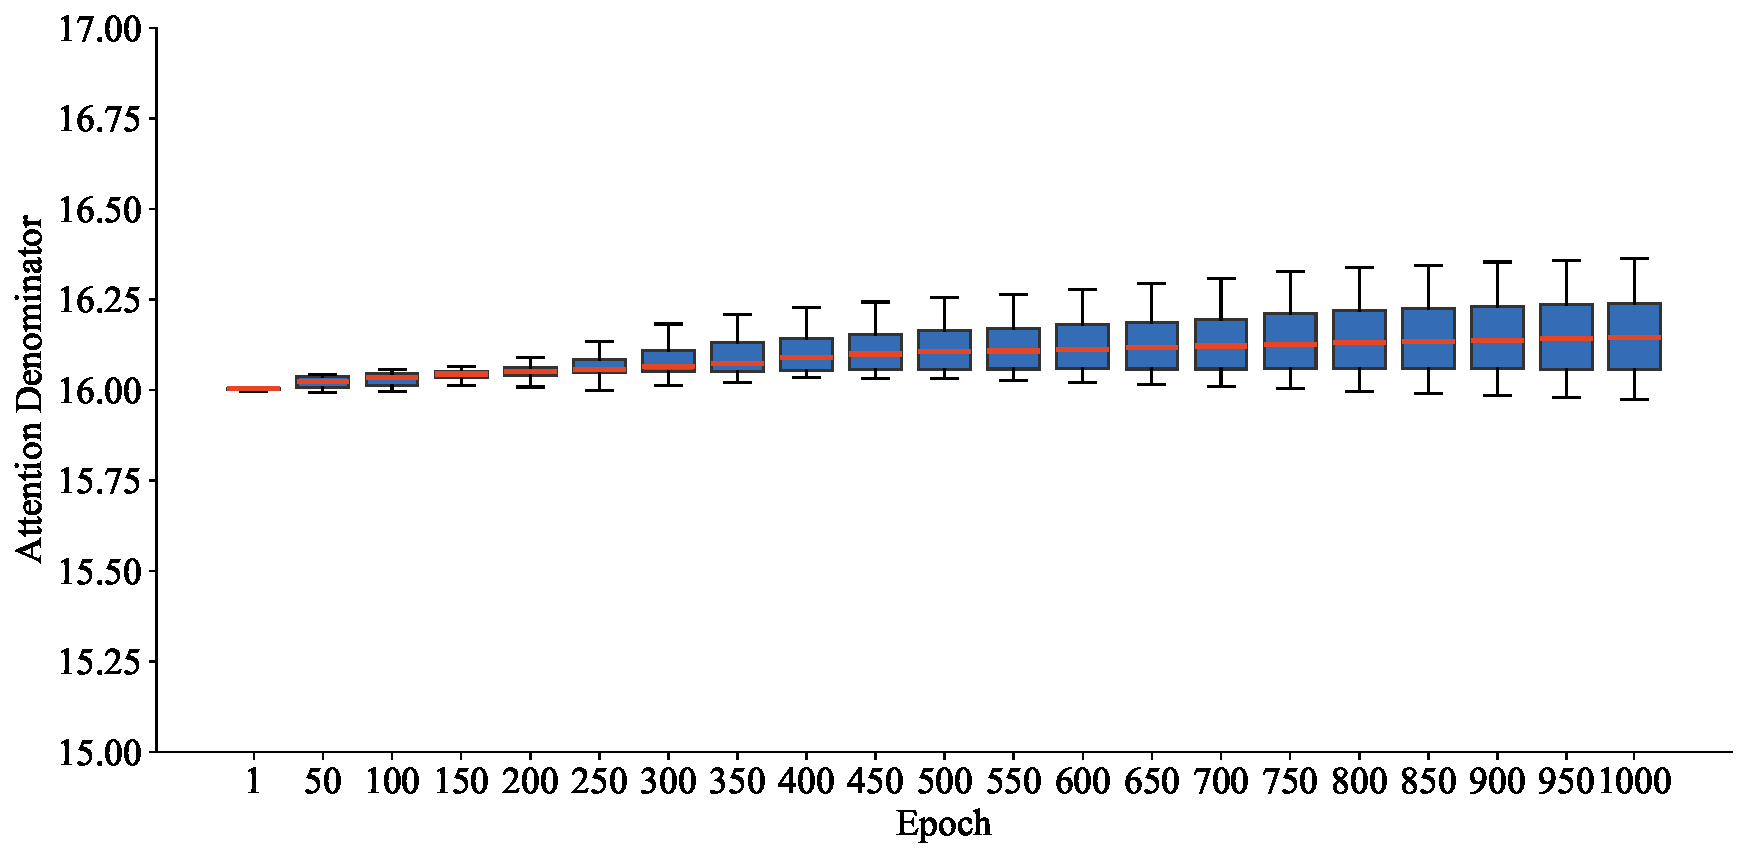
\includegraphics[width=\textwidth]{Figures/attention_denoms/attention_weights_aspirin.pdf}
        \caption{Aspirin}
    \end{subfigure}
    \hfill
    \begin{subfigure}{0.48\textwidth}
        \centering
        \includegraphics[width=\textwidth]{Figures/attention_denoms/attention_weights_ethanol.pdf}
        \caption{Ethanol}
    \end{subfigure}
    \begin{subfigure}{0.48\textwidth}
        \centering
        \includegraphics[width=\textwidth]{Figures/attention_denoms/attention_weights_napthalene.pdf}
        \caption{Napthalene}
    \end{subfigure}
    \hfill
    \begin{subfigure}{0.48\textwidth}
        \centering
        \includegraphics[width=\textwidth]{Figures/attention_denoms/attention_weights_toluene.pdf}
        \caption{Toluene}
    \end{subfigure}
    
    \caption{Learned attention denominators for aspirin of the MD17 dataset on \gls{atoms}. Each box contains 40 denominators (five layers \(\times\) eight heads).}
    \label{fig:attention_denoms}
\end{figure}

\section{Experimental Details}
\subsection{Software and Hardware Details}
All experiments were conducted using Python 3.12, NumPy 2.2.1 \cite{harris_array_2020}, PyTorch 2.5.1 \cite{paszke_pytorch_2019}, e3nn 0.5.6 \cite{geiger_e3nn_2022} and PyTorch Optimizer 3.5.0 \cite{kim_pytorch_optimizer_2021}. We use RDKit 2024.9.6 \cite{greg_landrum_rdkit_2012} and PubChemPy 1.0.4 in the construction of TG80. All training was performed on an NVIDIA Titan V (12 GB) running CUDA 12.4 on Ubuntu 24.04.

\subsection{\gls{atoms} Hyperparameters}
\label{sec:my_hyperparams}
We employ the same dataset splitting and discretization parameters reported in \textcite{xu_equivariant_2024} for the MD17 and \(N\)-body simulation tasks. We set the batch size to \(100\) to ensure complete batches and avoid Torch graph breaks, given our dataset sizes are multiples of \(100\). We reduce the AdamW \(\epsilon\) to \(1\times10^{-10}\) to avoid instability associated with the small gradients produced by zero-initialised weight matrices in early training \cite{jordan_nanogpt_2025}. We present a complete overview of our hyperparameters in \Cref{tab:gtno_hparams}.

\begin{table}[h]
    \centering
    \caption{Hyperparameters for \gls{atoms}. MD17 hyperparameters are shared across all molecules unless otherwise noted.}
    \label{tab:gtno_hparams}
    \begin{tabular}{cccc}
        Module & & MD17, RMD17 Value & TG80 Multitask \\
        % Module & & MD17, RMD17 Value & \(N\)-body Value & Multitask \\
        \midrule
        Training & & \\
        & Batch size & \( 100 \) & \( 192 \) \\
        & Epochs & \( 1000 \) & \(250\) \\
        & Max grad norm & \( 1.0 \) & \(1.0\) \\
        & Noise \(\sigma\) & \( 0.1 \) & \(0.1\) \\
        & \(\Delta t\) & \( 3000 \) & \( 10\ 000 \) \\
        & Timesteps \(P\) & \( 8 \) & \( 8 \) \\
        & Train/Val/Test & \( (500,3000,3000) \) & \( (500,3000,3000) \) \\
        \midrule
        Optimiser & & \\
        & Optimiser type & AdamW-AMSGrad\cite{loshchilov_decoupled_2017} & Muon \cite{jordan_muon_2024, kim_pytorch_optimizer_2021}  \\
        & Learning rate & \( 1\times10^{-3} \) & \( 1\times10^{-3} \) \\
        & \(\beta_1, \beta_2\) & \( 0.9, 0.999 \) & N/A \\
        & Weight decay & \( 1\times10^{-5} \) & \( 1\times10^{-5} \) \\
        & \(\epsilon\) & \( 1\times10^{-10} \) & \( 1\times10^{-5} \) \\
        \midrule
        Model & & \\
        & Embedding dim & \( 128 \) & \( 128 \) \\
        & No. layers & \( 5 \) & \( 5 \) \\
        & No. attention heads & \( 8 \) & \( 8 \) \\
        & No. output heads & \(1\) & \(8\) \\
        & Attention dropout & \( 0.2 \) & \( 0.2 \) \\
        & RoPE frequency & \( 1000 \) & \( 1000 \)\\
        & MLP layers & \( 2 \) & \( 2 \) \\
        & MLP activation & SwiGLU & SwiGLU \\
        & MLP dropout & \( 0.0 \) & \( 0.0 \) \\
        & Norm type & RMS norm & RMS norm \\
        & Learnable value residuals & True & True \\
        & Spherical harmonic bias & False & False \\
        \bottomrule
    \end{tabular}
\end{table}

\newpage
\subsection{EGNO Benchmarks}
\label{sec:egno_hyperparams}
We generated the \gls{egno} results reported in \Cref{tab:md17_results} with the same discretization parameters and hyperparameters as used in their experiments. We reduce the number of epochs from \(10\ 000\) to \(2\ 500\), and select the best validation loss epoch for testing. In the multitask case we increase batch size to 192, further reduce the number of epochs to 250, and employ the Muon optimiser as in \Cref{tab:gtno_hparams}.

\begin{table}[H]
    \centering
    \caption{Hyperparameter values for \gls{egno} across each benchmark dataset.}
    \label{tab:egno_hparams}
    \begin{tabular}{cccc}
        Module & & MD17, RMD17 Value & TG80 Multitask \\
        \midrule
        Training & & \\
        & Batch size & \( 100 \) & \( 192 \) \\
        & Epochs & \( 2500 \) & \( 250 \) \\
        & Max grad norm & Uncapped & Uncapped  \\
        & Noise \(\sigma\) & \( 0.1 \) & \(0.1\) \\
        & \(\Delta t\) & \( 3000 \) & \(10\ 000\) \\
        & Timesteps \(P\) & \( 8 \) & \(8\) \\
        & Train/Val/Test & \( (500,3000,3000) \) \\
        \midrule
        Optimiser & & \\
        & Optimiser type & Adam \cite{kingma_adam_2014} & Muon \cite{jordan_muon_2024, kim_pytorch_optimizer_2021}  \\
        & Learning rate & \( 1\times10^{-4} \) \\
        & \(\beta_1, \beta_2\) & \( (0.9, 0.999) \) & N/A \\
        & Weight decay & \( 1\times10^{-15} \) \\
        & \(\epsilon\) & \( 1\times10^{-8} \) \\
        \midrule
        Scheduler & & \\
        & Scheduler type & StepLR & StepLR \\
        & Step size & 2500 & 2500 \\
        & \(\gamma\) & 0.5 & 0.5 \\
        \midrule
        Model & & \\
        & Embedding dim & \( 64 \) & \( 64 \) \\
        & No. \gls{egno} layers & \( 5 \) & \( 5 \) \\
        & Temporal convolution activation & LeakyRELU & LeakyRELU \\
        & MLP layers & \( 2 \) & \( 2 \) \\
        & MLP activation & SiLU & SiLU \\
        & MLP dropout & \( 0 \) & \( 0 \) \\
        & Time embedding dim & 32 & 32 \\
        & Fourier modes & 2 & 2 \\
        \bottomrule
    \end{tabular}
\end{table}

\section{Proofs}
\subsection{Tensor Product Equivariance}
\label{appx:tpeq}
\newtheorem{tpeq}{Tensor product equivariance}
\begin{tpeq} \label{thm:tpeq}
    Let \( G \) be a group acting on \( \mathbb{R}^n \), and let \( V \) and \( W \) be vector spaces equipped with representations \( \rho: G \to GL(V) \) and \( \sigma: G \to GL(W) \), respectively. Suppose \( f: \mathbb{R}^n \to V \) and \( g: \mathbb{R}^n \to W \) are equivariant functions satisfying:
    \[
    f(h \cdot x) = \rho(h) f(x), \quad g(h \cdot x) = \sigma(h) g(x), \quad \forall h \in G.
    \]
    Then, their tensor product function
    \[
    (f \otimes g)(x) = f(x) \otimes g(x)
    \]
    is equivariant under the tensor product representation \( \rho \otimes \sigma \), i.e.,
    \[
    (f \otimes g)(h \cdot x) = (\rho \otimes \sigma)(h) (f(x) \otimes g(x)).
    \]
\end{tpeq}

\begin{proof}
    Applying \( h \in G \) to the input \( x \), we compute:
    \[
    (f \otimes g)(h \cdot x) = f(h \cdot x) \otimes g(h \cdot x).
    \]
    By the equivariance conditions of \( f \) and \( g \), we substitute:
    \[
    (f \otimes g)(h \cdot x) = (\rho(h) f(x)) \otimes (\sigma(h) g(x)).
    \]
    Since the tensor product of representations satisfies
    \[
    (\rho \otimes \sigma)(h) (v \otimes w) = (\rho(h) v) \otimes (\sigma(h) w),
    \]
    we recognize that
    \[
    (\rho(h) f(x)) \otimes (\sigma(h) g(x)) = (\rho \otimes \sigma)(h) (f(x) \otimes g(x)).
    \]
    Thus, we conclude:
    \[
    (f \otimes g)(h \cdot x) = (\rho \otimes \sigma)(h) (f(x) \otimes g(x)),
    \]
    proving that \( f \otimes g \) is equivariant under the tensor product representation.
\end{proof}

\begin{proof}[Proof of Proposition \ref{prop:kernel}]
Following \cite{gao_learning_2024} we may view our attention as a kernel integral transform by considering \(\mathbf{x}_i\) as being sampled from the continuum domain \(\Omega \subset \mathbb{R}^3\) for which we define the empirical measure with support on \(\{\mathbf{x}_i\}_{i=1}^N \subset \Omega\):
\begin{equation}
    {\mu_N} (\mathbf{x}) = \frac{1}{N} \sum_{i=1}^N \delta_{\mathbf{x}_i}, \qquad \int_\Omega g(\mathbf{x})d {\mu_N } (\mathbf x) =\frac{1}{N} \sum_{i=1}^N g(\mathbf{x}_i)
    \label{eq:measure}
\end{equation}
where \(\delta\) is the Dirac delta function \say{selecting} the values at \(\mathbf{x}_i\).
Given \gls{trope}-rotated query and key maps \(\tilde{q}_\theta(\mathbf{z})=R_{p(\mathbf{z})}q_\theta(\mathbf{z}_j)\), \(\tilde{k}^F(\mathbf{x}_i)=R_{p(\mathbf{x}_i)}k_\theta^F(\mathbf{x}_i)\) we form the data-dependent kernel for feature \(F\):
\begin{equation}
    \kappa_{\theta}^F(\mathbf{z}, \mathbf{x}_i)
    = 
    \frac{
      \exp\bigl(\langle \tilde q(\mathbf{z}),\,\tilde k^F(\mathbf{x}_i)\rangle \;/\;\sqrt{d_{h}}\bigr)
    }{
      \displaystyle
      \int_{\Omega}
        \exp\bigl(\langle \tilde q(\mathbf{z}_{j}),\,\tilde k^F(\mathbf{x}')\rangle \;/\;\sqrt{d_{h}}\bigr)
        \,d\mu_{N}(\mathbf{x}')
    }\,.
\end{equation}
Thus, for any \(F \in \mathcal{F}\) we may represent our cross-attention as the kernel integral operator:
\begin{equation}
    \bigl(\mathcal{K}_\theta^F \mathbf{v}^F\bigr)(\mathbf{z}) = \int_{\Omega} \kappa_\theta^F\bigl(\mathbf{z}, \mathbf{x}\bigr)\,\mathbf{v}^F(\mathbf{x})\,\mathrm{d}\mu_N(\mathbf{x}),
    \qquad
    \int_\Omega\kappa_\theta^F(\mathbf{z},\mathbf{x})\, d \mu_N(\mathbf{x})=1,
\end{equation}
which is row-stochastic under the measure in \Cref{eq:measure}.     
\end{proof}